\chapter{用 AI 辅助数据可视化}

生态学专业的研究生林悦刚整理完一份南极帕默群岛（Palmer Archipelago）三种企鹅繁殖成体的形态测量数据表。为了在组会汇报和论文“研究对象”一节展示三种企鹅的体重差异，她打开一个支持对话的数据可视化工具，上传表格后输入了一句：“帮我画一张专业的企鹅体重比较图，要符合期刊风格。”几秒钟后，屏幕上出现了一张配色明快、排版端正的柱状图：三根彩色柱子代表三种企鹅，每根柱子顶端各立着一小段黑色误差线。

初看之下，这张图干净利落，似乎可以直接放进手稿。然而在组会上，导师接连问出四个最基本的问题，林悦却一个也答不上来：第一，柱顶那截短短的误差线究竟表示标准差（SD）、标准误（SEM）还是 95\% 置信区间？第二，每根柱子背后分别汇总了多少条测量记录，表里的缺失值被工具怎么处理了？第三，企鹅体重存在明显的雌雄二态性，把雌雄混在一根柱子里算均值，掩盖了多少物种内部的性别差异？第四，为什么前两种企鹅的平均体重只相差三十多克，在另一张自动缩放纵轴的草图里却看起来差了将近一倍？

数据图在论文中不是点缀版面的装饰画，而是直接支撑科学结论的定量证据。对话式可视化工具可以帮我们省去查阅绘图函数语法的繁琐时间，但只要输入的指令含糊不清，工具就会在后台替作者做出一连串未经授权的统计汇总与视觉编码决定。因此，面对任何一张 AI 生成或辅助修改的数据图，我们要问的第一个问题从来不是“这张图好不好看”，而是“这张图对不对、诚不诚实、能不能经得起逐项核对”。本章从读懂一张原始数据表开始，系统拆解如何用 AI 工具辅助制作、修改并严格核验科研数据图。

\section{先读表，再选图}

拿到数据表后直接拖进绘图工具并让 AI“推荐最合适的图”，是造成后续反复返工甚至发表错误图表的常见根源。软件只能读取列名和数值格式，却看不到数据背后的采样过程与实验设计。在动手画图之前，作者必须先替 AI 完成四项“读表”工作。

\textbf{第一，确认每一行代表什么观测单位。}这是最容易被 AI 误判、也最容易被作者略过的一步。本章主案例使用南极帕默站长期生态研究项目（Palmer Station LTER）采集、由 Horst 等（2020）整理发布的公开企鹅数据集（\texttt{palmerpenguins} v0.1.0，CC0 许可；原始生态学研究见 Gorman 等，2014）。清理后的数据表 \texttt{penguins.csv} 共 344 行、8 列。如果你把这张表传给 AI 并直接提问“表里有多少只企鹅”，AI 会毫不犹豫地回答“344 只”。但只要查阅原始数据包说明就会发现，原始记录中的个体编号（\texttt{Individual ID}，如 \texttt{N21A1}）采用的是按筑巢位置编码的规则，在 344 行记录中有 60 个“物种 + 个体编号”组合在 2007—2009 三个研究季之间重复出现。单凭清理后的表格，未经逐一核实原始野外记录，并不能直接断言“每一行都是一只不同的企鹅个体”。因此，最严谨、保守的表述是把每一行定义为\textbf{一条繁殖成体的形态测量记录}，并在任务书和图注中明确写为“$n = \text{记录数}$”。AI 可以快速统计表格行数，却看不出编码规则背后的生态学采样逻辑，这种界定必须由作者亲自完成。

\textbf{第二，清点变量类型、物理单位与记录精度。}打开表格后，应逐列区分哪些是分类分组变量，哪些是连续测量变量，哪些是时间或批次标记，并整理成数据字典（表~\ref{tab:ch05-dict}）。这里需重点防范两类陷阱：一是\textbf{用整数编码的批次标记}，如表中的 \texttt{year} 列取值为 2007、2008、2009，在软件眼里它是标准数值列，若不加说明，自动绘图功能常会把它当成连续测量变量去算“平均年份”或画进相关性矩阵，而实际上它只是三个采样研究季的批次标记；二是\textbf{原始测量的最小刻度}，如鳍肢长度记录到整数毫米，体重（\texttt{body\_mass\_g}）在野外称重时以 $25\ \text{g}$ 或 $50\ \text{g}$ 为最小刻度记录整数，后续若在图上标出三位小数就会制造伪精度。

\begin{table}[htbp]\centering\footnotesize
\setlength{\tabcolsep}{3pt}
\renewcommand{\arraystretch}{1.15}
\caption{帕默企鹅数据集（\texttt{penguins.csv}，共 344 行）的数据字典。}\label{tab:ch05-dict}
\begin{tabularx}{\linewidth}{@{}l>{\raggedright\arraybackslash}p{26mm}cY c@{}}
\toprule
\textbf{列名} & \textbf{类型} & \textbf{单位} & \textbf{说明} & \textbf{缺失} \\
\midrule
\texttt{species} & 分类（3 水平） & — & 阿德利（Adelie）/ 帽带（Chinstrap）/ 巴布亚（Gentoo） & 0 \\
\texttt{island} & 分类（3 水平） & — & Biscoe / Dream / Torgersen；巴布亚仅见于 Biscoe，帽带仅见于 Dream，阿德利三岛均有 & 0 \\
\texttt{bill\_length\_mm} & 连续 & mm & 嘴峰长度（沿嘴峰上缘测量的喙长） & 2 \\
\texttt{bill\_depth\_mm} & 连续 & mm & 嘴峰深度（闭合喙部的竖直高度） & 2 \\
\texttt{flipper\_length\_mm} & 连续（整数） & mm & 鳍肢长度 & 2 \\
\texttt{body\_mass\_g} & 连续（整数） & g & 体重（野外记录到 $25\ \text{g}$ 或 $50\ \text{g}$ 量级） & 2 \\
\texttt{sex} & 分类（2 水平） & — & \texttt{female}（雌）/ \texttt{male}（雄） & 11 \\
\texttt{year} & 整数 & — & 2007 / 2008 / 2009，研究季标记，不是测量值 & 0 \\
\bottomrule
\end{tabularx}
\end{table}

\textbf{第三，核查缺失值（NA）的数量与重叠关系。}表~\ref{tab:ch05-dict} 中四个形态测量列各缺 2 行（记作字符串 \texttt{NA}），而性别列有 11 行缺失；进一步核对可知，体重缺失的那 2 行同时也缺失性别。这一事实直接决定了不同分析视角下的有效样本量：如果只按物种汇总体重或嘴峰尺寸，剔除测量值缺失的 2 行后有效记录数为 $n = 342$；如果按“物种 $\times$ 性别”交叉分组分析体重，则需剔除性别或体重为 \texttt{NA} 的共 11 行，保留有效记录数 \textbf{$n = 333$}。若不在指令中写明剔除规则，绘图工具要么静默删行而不报告样本量，要么把字符串 \texttt{"NA"} 当成第三个性别组画在横轴上。

\textbf{第四，识别分类混杂与研究设计。}注意表~\ref{tab:ch05-dict} 中 \texttt{island} 列的分布：Torgersen 岛全部是阿德利企鹅（52 条），Biscoe 岛只有阿德利（44 条）和体型庞大的巴布亚企鹅（124 条），Dream 岛则只有阿德利（56 条）和帽带企鹅（68 条）。若不看数据字典就直接画“三个岛的企鹅平均体型对比”，Biscoe 岛会显得格外重——但这并非岛屿环境造就的同种差异，而是因为巴布亚企鹅只在该岛采样。同样，不同行之间究竟是独立组、配对前后测、重复测量还是时间序列，直接决定了候选图型家族与图上必须保留的信息（表~\ref{tab:ch05-01}）。

\begin{table}[htbp]\centering\footnotesize
\setlength{\tabcolsep}{3pt}
\renewcommand{\arraystretch}{1.15}
\caption{研究设计与数据结构对应的候选图型及常见 AI 默认错误。}\label{tab:ch05-01}
\begin{tabularx}{\linewidth}{@{}>{\raggedright\arraybackslash}p{28mm}>{\raggedright\arraybackslash}p{25mm}YY@{}}
\toprule
\textbf{研究设计 / 数据结构} & \textbf{候选图型} & \textbf{必须保留的信息} & \textbf{常见 AI 默认错误} \\
\midrule
少数独立组的连续测量（每组 $n < \text{约 }30$） & 散点 + 均值/中位数、箱线 + 散点 & 所有观测点、每组 $n$ & 只画均值柱 + SEM \\
独立组、$n$ 较大 & 箱线图、小提琴图、云雨图 & 分布形状、$n$、离群值 & 小提琴图把 $n$ 隐藏；核密度平滑过度 \\
配对 / 前后测 & 配对点线图、差值图 & 配对键、个体轨迹、方向不同的对象 & 当作两独立组；删“异常”对象 \\
重复测量多个时间点 & 个体轨迹 + 均值线；分面 & 个体 ID、时间间隔真实比例 & 时间当分类变量、等距排布不等距时间 \\
时间序列 & 折线（连续时间轴） & 缺测/插补标记、测量方法变化 & 双纵轴；平滑掉季节信号不说明 \\
两个连续变量 & 散点（+分组颜色/形状）、必要时拟合线 & 分组结构、$n$、拟合方法 & 全体一条回归线；图上堆 $p$ 值 \\
矩阵 / 二维场 & 热图（感知均匀色图） & 色标、单位、数值范围 & 彩虹色图；色标不标单位 \\
\bottomrule
\end{tabularx}
\end{table}

\section{分组比较：同一份数据，四种画法}

比较几个独立分组的连续测量值时，最核心的权衡在于：\textbf{把原始观测汇总到什么程度？}汇总得越激进，画面越简单，被隐藏的数据结构也越多。我们取剔除 2 条体重缺失记录后的 $n = 342$ 条企鹅记录（阿德利 151、帽带 68、巴布亚 123），用四种常见图型展示同一份数据（图~\ref{fig:ch05-01}）。全章企鹅图统一采用对色觉异常友好的 Okabe–Ito 配色：阿德利橙色（\texttt{\#E69F00}）、帽带天蓝（\texttt{\#56B4E9}）、巴布亚蓝绿（\texttt{\#009E73}）。

\begin{figure}[htbp]\centering
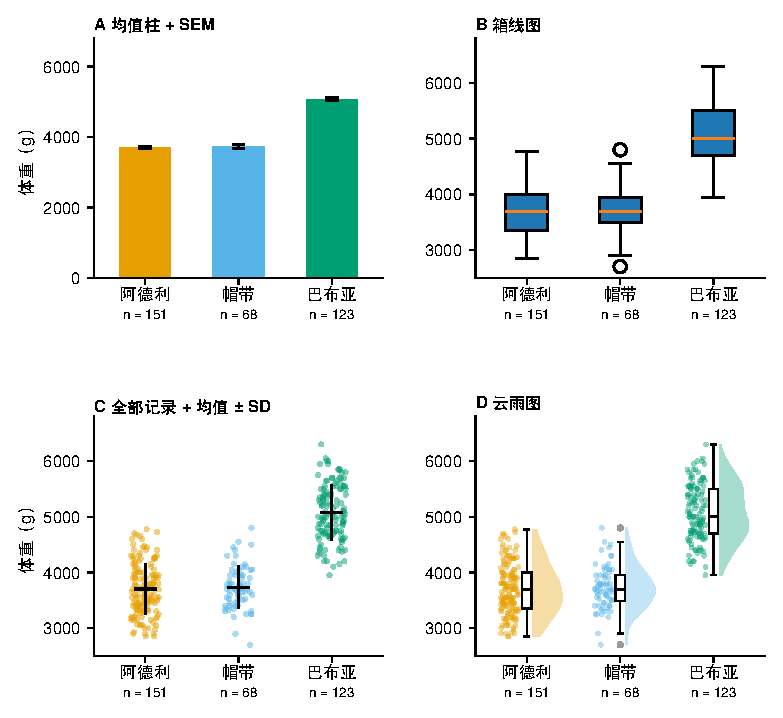
\includegraphics[width=\linewidth]{figures/ch05/ch05-01-group-forms-zh.pdf}
\caption{同一组数据的四种表达。三种企鹅体重（palmerpenguins，$n = 342$ 条记录；剔除体重缺失 2 条）。A 均值柱与 $\pm 1\ \text{SEM}$；B 箱线图（须为 $1.5$ 倍四分位距）；C 全部记录与均值 $\pm 1\ \text{SD}$；D 云雨图（核密度、箱线与原始点）。A 只呈现 6 个数，看不出帽带企鹅的记录数不到阿德利的一半，也看不到分布形状。}\label{fig:ch05-01}
\end{figure}

对照图~\ref{fig:ch05-01} 的四个面板，可以清楚看到每种画法的得失：

\begin{itemize}
\item \textbf{面板 A（均值柱 + SEM）：把 342 条记录压缩成 6 个数。}面板 A 的纵轴诚实地从 $0\ \text{g}$ 起步，但它只给出了 3 个均值（$3700.7\ \text{g}$、$3733.1\ \text{g}$、$5076.0\ \text{g}$）和 3 个均值标准误（$37.3\ \text{g}$、$46.6\ \text{g}$、$45.5\ \text{g}$）。柱顶的 SEM 误差线在数千克尺度上短得几乎缩成一条黑线。若不在横轴下方专门标出 $n$，三根等宽的柱子完全掩盖了帽带企鹅记录数（$n=68$）还不到阿德利（$n=151$）一半的事实；同时，$0\text{--}2700\ \text{g}$ 之间没有任何成体企鹅记录，实心柱却占去近半画幅，真正有数据分布的区间反而被挤压。Weissgerber 等（2015）指出，完全相同的柱子加误差线可能对应正态、偏态、双峰或含极端值的分布，中小样本比较应优先展示原始观测点。

\item \textbf{面板 B（箱线图）：展示分位数与离群点，但仍隐藏 $n$ 与亚群。}面板 B 将纵轴聚焦在 $2500\text{--}6800\ \text{g}$（箱线图不靠柱体面积编码数值，纵轴可不从 0 开始）。箱内橙线为中位数（阿德利与帽带均为 $3700\ \text{g}$，巴布亚为 $5000\ \text{g}$），箱体上下缘为第一、三四分位数（四分位距 IQR），须线延伸至 $1.5 \times \text{IQR}$。此时面板 A 隐藏的一个特征显露出来：帽带企鹅上下两端各有一个超出 $1.5 \times \text{IQR}$ 的空心圆离群点（最低值 $2700\ \text{g}$ 与最高值 $4800\ \text{g}$）。但箱体宽度本身仍不反映样本量差异，且当组内包含雌雄两个亚群时，单一箱体依然会把潜在的双峰结构合并成一个长方形。

\item \textbf{面板 C（全部记录 + 均值 $\pm$ SD）：把每一个观测点还给读者。}面板 C 将 342 条记录全部画成半透明散点，并叠加黑色短横线（均值）与竖线（$\pm 1\ \text{SD}$）。读者一眼就能读出三层信息：第一，中间天蓝色的帽带企鹅点云明显比两侧稀疏；第二，各物种内部个体体重跨度达近两千克（阿德利 $2850\text{--}4775\ \text{g}$，帽带 $2700\text{--}4800\ \text{g}$，巴布亚 $3950\text{--}6300\ \text{g}$），均值 $\pm 1\ \text{SD}$ 竖线如实反映了点云的主体离散宽度；第三，两端极值点自然呈现在点云上下边界，无需依赖人为须线阈值即可看清。

\item \textbf{面板 D（云雨图，Raincloud plot）：分布轮廓、箱线与原始点三合一。}按 Allen 等（2019）的设计，面板 D 在每组左侧画横向抖动的原始点（“雨”），中间放窄白底箱线图，右侧画截断在各组极值范围内的半边核密度估计曲线（“云”）。右侧平滑的密度轮廓能直观揭示点云内部的聚集形态——例如巴布亚企鹅（右侧蓝绿）的密度曲线在 $4700\ \text{g}$ 与 $5500\ \text{g}$ 附近呈现出宽肩形态，恰好提示该物种内部包含雌雄两个亚群。
\end{itemize}

据此可以定下一条清晰的选图原则：\textbf{当每组样本量较小或中等（几条至百余条）时，优先展示全部原始点（面板 C 或 D）；当每组样本量极大、散点完全重叠成墨团时，使用箱线图、小提琴图或云雨图，并务必在横轴下方标明每组的 $n$。}在 \scidraw{} 科学可视化（\sdtool{sci-vis}）中要求展示原始散点时，必须在对话指令中明确说明\textbf{随机抖动只改变横坐标，不改变纵坐标数值}：

\begin{Prompt}
改为分组散点图：横轴为物种（阿德利、帽带、巴布亚），纵轴为体重（g），范围 2500–6800。
显示全部 342 条记录的原始点，点只在横向轻微随机抖动（不超过组间距的 15%）以减少重叠，
纵向测量数值绝不改变。每组叠加均值（短横线）与 ± 1 SD（竖线），横轴下方标出每组 n。
\end{Prompt}

\section{误差线到底表示什么}

对比图~\ref{fig:ch05-01} 面板 A 与面板 C：同样是阿德利企鹅的 151 条体重记录，为什么面板 A 柱顶的误差线只有短短几十克，而面板 C 点云中的误差线却长得多？因为面板 A 画的是均值标准误（SEM），面板 C 画的是样本标准差（SD）。把不同误差线混为一谈，或干脆不说明误差线类型，是科研论文配图的高发错误（Cumming 等，2007；Krzywinski 与 Altman，2013）。

三种常见误差线回答的是三个截然不同的问题（表~\ref{tab:ch05-err}）：

\begin{table}[htbp]\centering\footnotesize
\setlength{\tabcolsep}{2.5pt}
\renewcommand{\arraystretch}{1.15}
\caption{三种常见误差线的含义及在企鹅体重数据（$n=342$：阿德利 151、帽带 68、巴布亚 123）中的实际半宽对比。}\label{tab:ch05-err}
\begin{tabularx}{\linewidth}{@{}>{\raggedright\arraybackslash}p{18mm}>{\raggedright\arraybackslash}p{22mm}Yccc@{}}
\toprule
\textbf{误差线类型} & \textbf{计算公式} & \textbf{回答的科学问题与随 $n$ 变化的规律} & \textbf{阿德利} & \textbf{帽带} & \textbf{巴布亚} \\
\midrule
样本标准差（SD） & $s = \sqrt{\frac{\sum (x_i - \bar{x})^2}{n-1}}$ & \textbf{描述离散度：}个体测量值本身相差多大？随 $n$ 增大趋于稳定，不会因多测样本而变短 & $458.6\ \text{g}$ & $384.3\ \text{g}$ & $504.1\ \text{g}$ \\
均值标准误（SEM） & $\text{SEM} = s / \sqrt{n}$ & \textbf{估计精度：}样本均值离总体均值多远？随 $\sqrt{n}$ 增大而迅速缩短，不反映个体离散度 & $37.3\ \text{g}$ & $46.6\ \text{g}$ & $45.5\ \text{g}$ \\
95\% 置信区间半宽 & $t_{0.975,\,n-1} \times \text{SEM}$ & \textbf{区间估计：}总体均值的 95\% 估计区间半宽（大样本下约为 SEM 的 2 倍） & $73.7\ \text{g}$ & $93.0\ \text{g}$ & $90.0\ \text{g}$ \\
\bottomrule
\end{tabularx}
\end{table}

从表~\ref{tab:ch05-err} 的实测数据应牢记三条准则：
第一，\textbf{同一组数据的 SD 与 SEM 可相差十倍以上}。阿德利企鹅的 $\text{SD} = 458.6\ \text{g}$，除以 $\sqrt{151} \approx 12.29$ 后得到的 $\text{SEM}$ 仅为 $37.3\ \text{g}$，$95\%\ \text{CI}$ 半宽约为 $73.7\ \text{g}$。若想向读者展示个体体重本身的波动范围，必须用 SD（或四分位距）；若想展示总体均值的估计区间，优先用 95\% CI，切勿为了追求“误差线短、显得数据漂亮”而选用 SEM。
第二，\textbf{所有误差线都必须在图例或图注中写明统计类型与每组 $n$}，只有同时给出类型和 $n$，读者才能准确解读并在需要时换算。
第三，\textbf{不能凭误差线“重不重叠”直接断定差异是否显著}（Cumming 等，2007；Krzywinski 与 Altman，2013）。当图上画的是 $\pm 1\ \text{SD}$ 时，两条误差线大幅重叠，两组均值仍可能高度显著不同；当画的是独立样本的 $\pm 1\ \text{SEM}$ 时，即便两条误差线刚刚不重叠，双侧 $p$ 值仍大于 $0.05$（两独立且样本量相近的大样本，SEM 误差线需留出约 0.5–1 倍 SEM 的空隙，或两条 95\% CI 重叠不超过单侧臂长的约四分之一，才大致对应 $p \le 0.05$）。

由于许多 AI 绘图工具默认绘制最短的 SEM 且不加说明，作者在 \sdtool{sci-vis} 中必须明确点名误差线统计量：

\begin{Prompt}
误差线请统一使用样本标准差（± 1 SD，ddof = 1），不要使用标准误（SEM）。
在图例中写明“横线：均值；竖线：± 1 SD”，在横轴每组下方标注样本量 n，不画星号或 p 值。
\end{Prompt}

\section{配对与重复测量}

当两列数值来自同一批研究对象在处理前后的两次测定（或同一样点在两个时期的复测），数据就具有一一对应的\textbf{配对结构（paired structure）}。我们延续第 1、2 章使用的模拟教学数据集（\texttt{paired-example.csv}，CC BY 4.0）：8 个虚构对象（\texttt{SIM01}–\texttt{SIM08}），前测均值 $13.125\ \text{a.u.}$，后测均值 $16.5\ \text{a.u.}$，各对象差值（后测 $-$ 前测）依次为 $+4, +3, +4, -1, +4, +5, +4, +4$，均值差 $3.375\ \text{a.u.}$。图~\ref{fig:ch05-03} 对比了这份配对数据的三种画法。

\begin{figure}[htbp]\centering
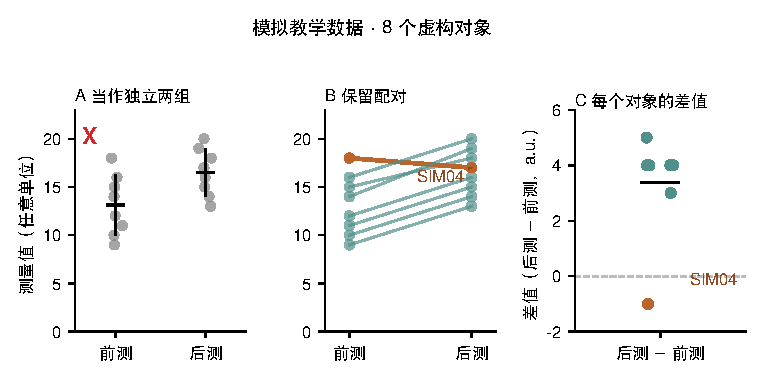
\includegraphics[width=\linewidth]{figures/ch05/ch05-03-paired-views-zh.pdf}
\caption{配对数据的三种画法（模拟教学数据）。8 个虚构对象各测量两次。A 把两列当作独立组，配对信息消失，读者可能以为有 16 个对象；B 保留每个对象的前后连线，\texttt{SIM04} 下降可见；C 直接展示每个对象的差值，7 个为正、1 个为负，均值差 $3.375\ \text{a.u.}$。未进行显著性检验。}\label{fig:ch05-03}
\end{figure}

观察图~\ref{fig:ch05-03} 三个面板的实际画面：
\begin{itemize}
\item \textbf{面板 A（当作独立两组，左上角标红色“X”）：丢失配对的错误画法。}面板 A 只把前测和后测画成两列孤立的灰色散点与均值 $\pm\ \text{SD}$。这会造成两个严重后果：一是画面上出现 16 个孤立散点，读者很容易误以为实验测量了 16 个独立对象；二是个体初始基线跨度很大（前测从 $9$ 到 $18$），组间基线差异完全淹没了组内变化，两列点的纵向区间大幅重叠，根本看不出每个对象在后测中究竟是升是降。
\item \textbf{面板 B（保留配对的斜率图 / 配对点线图）：呈现个体轨迹与逆向个体。}面板 B 用线段把同一对象的前测值与后测值连接起来。画面传达的信息瞬间清晰：8 个对象中有 7 条青绿色连线平行向右上倾斜（增幅 $+3$ 至 $+5$），唯独用暖棕色加粗标出的 \texttt{SIM04} 从前测最高基线 $18$ 降至后测的 $17$（变化量 $-1$）。当读者既关心对象的初始基线水平（例如 \texttt{SIM04} 基线最高，提示可能存在天花板效应），又关心变化方向是否一致时，应选用面板 B。
\item \textbf{面板 C（每个对象的差值图）：直接回答“变化了多少”。}当研究问题直接聚焦于“处理带来了多大的变化量”时，面板 C 以个体差值（后测 $-$ 前测）为纵轴画出 8 个差值点，用黑色短横线标出均值差 $3.375\ \text{a.u.}$，并在 $y = 0$ 处画一条灰色虚线作为“无变化”参考基线。7 个青绿色点落在零线上方 $+3$ 至 $+5$ 处（$+4$ 处的 5 个点横向微幅错开），棕色点 \texttt{SIM04} 落在零线下方 $-1$ 处。这里有一条硬性规范：\textbf{差值图的纵轴（本图为 $-2$ 至 $6$）必须包含 $0$ 并画出零参考线}，因为零线是判断增减方向的分界线。
\end{itemize}

使用 AI 工具绘制配对数据时，作者必须重点防范两项风险：一是工具忽略对象编号列（\texttt{sample\_id}），默认把前后两列当成两个独立组画成面板 A；二是当指令中出现“清理数据并突出主要趋势”等模糊表述时，部分自动脚本会把唯一逆向下降的 \texttt{SIM04} 当作“异常值”静默删掉。因此任务书中必须明确规定：“按 \texttt{sample\_id} 连线保留配对关系，完整保留全部 8 个对象，严禁剔除任何逆向变化或极端个体。”

\section{时间序列与双纵轴}

时间序列数据具有严格的先后顺序与时间比例，作图底线有两条：\textbf{横轴必须按真实时间间隔连续映射，数据说明中的插补与观测变更必须在图上留痕。}

本节使用地球与环境科学领域的经典观测记录——夏威夷莫纳罗亚（Mauna Loa）观测站大气 $\text{CO}_2$ 干空气摩尔分数月均值序列（Keeling，1960；由美国国家海洋和大气管理局全球监测实验室 NOAA GML 的 Xin Lan 博士与斯克里普斯海洋研究所 Scripps 的 Ralph Keeling 博士共同维护，公有领域，采用 WMO X2019 标度）。本案例锁定的公开数据快照（文件头创建日期为 2026 年 10 月 9 日）包含自 1958 年 3 月（$315.71\ \text{ppm}$）至 2026 年 9 月（$426.07\ \text{ppm}$）共 823 行月度记录，全时段最低月均值为 $312.42\ \text{ppm}$，最高月均值为 $432.34\ \text{ppm}$（2026 年 5 月）。图~\ref{fig:ch05-04} 展示了该序列的标准画法。

\begin{figure}[htbp]\centering
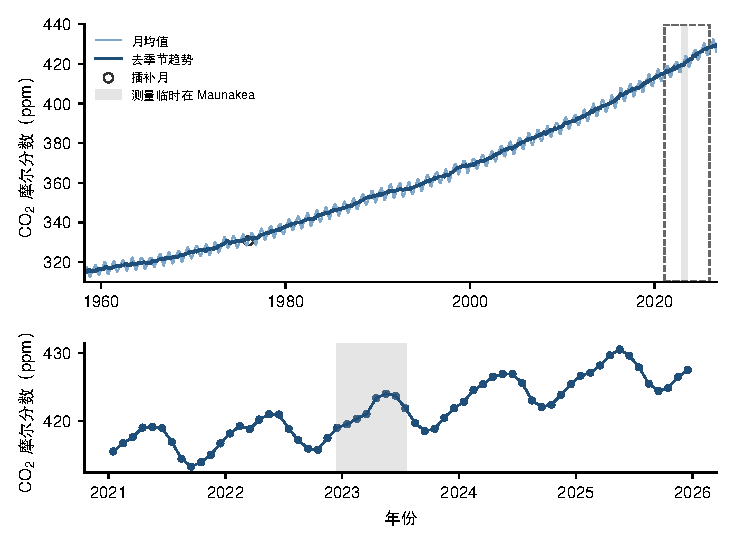
\includegraphics[width=\linewidth]{figures/ch05/ch05-04-co2-series-zh.pdf}
\caption{Mauna Loa 大气 $\text{CO}_2$ 月均值（1958 年 3 月至 2026 年 9 月快照）。上图（全时段）：细线为月均值，粗线为 NOAA 提供的去季节趋势值；空心圆为数据说明中的插补月（1975 年 12 月）；灰带为火山喷发后测量临时移至 Maunakea 的时段（2022 年 12 月至 2023 年 7 月）；右侧虚线框标出下图的放大范围。下图为最近 5 个完整年（2021—2025 年）的局部放大，可见明显的季节振荡。数据：NOAA GML（X.\ Lan）与 Scripps（R.\ Keeling），文件创建日期 2026 年 10 月 9 日；1974 年 5 月前为 Scripps 数据。}\label{fig:ch05-04}
\end{figure}

核对图~\ref{fig:ch05-04} 的上下两个面板，可以总结出时间序列作图的四项规范：
\begin{enumerate}
\item \textbf{连续数值时间轴：}横轴直接使用表中的十进制年份（\texttt{decimal date}），保证每一年、每个月的水平间距严格等比例，绝不把日期当成无序分类标签排列。
\item \textbf{原始观测与趋势分层并列：}上图同时绘出浅蓝细线（每月实测均值 \texttt{average}）与深蓝粗线（NOAA 官方去季节趋势 \texttt{deseasonalized}），不私自用未经说明的平滑滤波替掉原始波动。
\item \textbf{局部放大展示高频周期：}全时段近 70 年尺度下季节波动被压缩成密集细齿，因此上图右侧用虚线矩形框标出最近 5 个完整年（2021—2025 年），并在下图按 $2:1$ 高度比放大展示每月一个实心点的折线，清晰呈现北半球陆地植被生长季驱动的季节振荡（每年 5 月前后达峰、9—10 月见谷）。
\item \textbf{标出数据文件头注释中的特殊时段：}许多研究者读入 CSV 时直接跳过开头的 \texttt{\#} 注释行，却漏掉了关键背景。Mauna Loa 文件头注释明确记载：第一，1974 年 5 月前数据来自 Scripps，而自 1974 年 5 月 NOAA 独立观测以来，仅 1975 年 12 月因仪器故障无有效观测天数（\texttt{ndays} 为 $-1$），其数值为插补值——上图在 1975 年 12 月处专门用空心圆标出“插补月”；第二，2022 年 11 月底莫纳罗亚火山喷发切断站点供电与道路，2022 年 12 月至 2023 年 7 月测量临时移至约 21 英里外的莫纳克亚（Maunakea）山顶进行——上下两图均用浅灰色半透明竖带标出该时段。这些注释信息 AI 无法仅凭数字列猜出，必须由作者研读说明后要求标注。
\end{enumerate}

当需要同时展示两个量纲或量级不同的时间序列时，最常见的误导是\textbf{双纵轴（dual y-axes）}。我们取 Mauna Loa 完整日历年（1959—2025 年，共 67 年）的 12 个月均值算出年均浓度，再由相邻两年年均值之差算出 1960—2025 年（共 66 个值）的“年增长量”（单位：$\text{ppm/年}$；实测最小 $0.42$、最大 2024 年 $3.52\ \text{ppm/年}$，1960 年 $0.93$、2025 年 $2.74\ \text{ppm/年}$；注意这是相邻年均值之差，与 NOAA 官方按年末去季节值计算的年增长率算法不同，图注必须说明）。图~\ref{fig:ch05-06} 对比了双纵轴反例与上下分面正例。

\begin{figure}[htbp]\centering
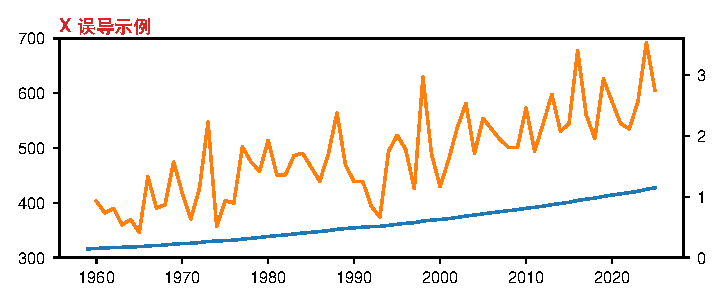
\includegraphics[width=\linewidth]{figures/ch05/ch05-06-dual-axis-bad-zh.pdf}\\[4pt]
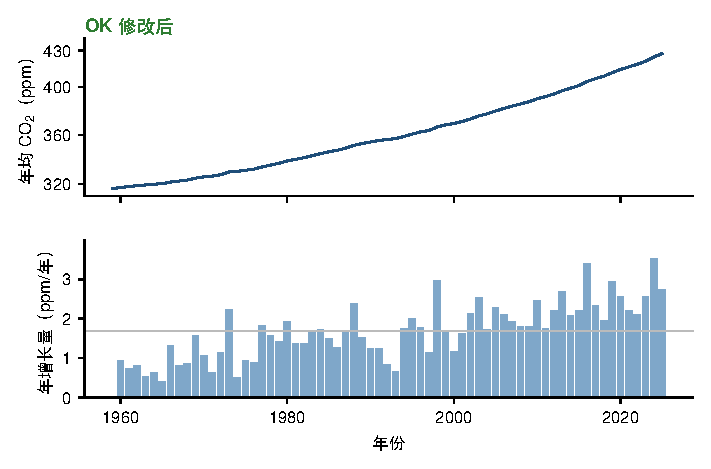
\includegraphics[width=\linewidth]{figures/ch05/ch05-06-dual-axis-good-zh.pdf}
\caption{双纵轴与分面（上为教学用错误示范）。上：年均 $\text{CO}_2$ 与年增长量共用一张图、两条纵轴，范围被人为选择，两线的相对位置没有意义。下：两个量各占一个面板，共享时间轴，增长量纵轴从 0 开始。年均值由 NOAA 月均值计算（仅完整年，1959—2025）；年增长量为相邻两年年均值之差，算法与 NOAA 官方增长率不同。}\label{fig:ch05-06}
\end{figure}

在图~\ref{fig:ch05-06} 上图（\texttt{X 误导示例}）中，左轴将年均浓度（蓝线）的范围人为拉大到 $300\text{--}700\ \text{ppm}$，把原本陡峭上升的浓度曲线压扁在底部；右轴将年增长量（橙线）设为 $0\text{--}3.6$ 撑满画幅，且左右两轴均无标题与单位。双纵轴的致命缺陷在于：\textbf{两条纵轴的起点与缩放比例可被任意调节}，作图者只需改动任一轴的范围，就能让两条线在任意年份“交叉”或“平行”，诱导读者从毫无物理意义的视觉交点中读出虚假关系。下图（\texttt{OK 修改后}）改用共享年份横轴的上下两个独立面板：上面板画年均浓度折线（$310\text{--}440\ \text{ppm}$），下面板用从 $0$ 开始的柱状图画年增长量（$0\text{--}4.0\ \text{ppm/年}$）并标出 1960—2025 年平均增长量参考线（浅灰横线，约 $1.69\ \text{ppm/年}$），既诚实保留各自量纲与基线，又方便顺着同一时间轴上下比对。

\section{散点与相关：分组变量会改变结论}

考察两个连续测量变量的关系时，若不向工具交代分类分组结构，AI 默认画出的“全体样本一条回归线”甚至会给出方向完全相反的结论。图~\ref{fig:ch05-08} 以企鹅嘴峰长度（\texttt{bill\_length\_mm}）与嘴峰深度（\texttt{bill\_depth\_mm}，剔除缺失 2 行后 $n = 342$）展示了教科书级的\textbf{辛普森悖论（Simpson's paradox）}。

\begin{figure}[htbp]\centering
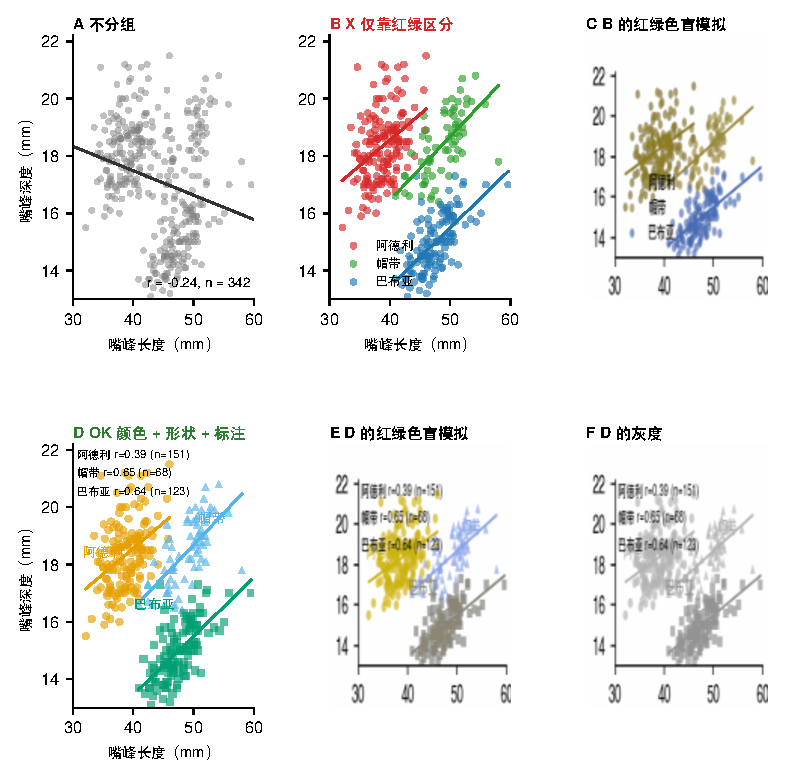
\includegraphics[width=\linewidth]{figures/ch05/ch05-08-scatter-cvd-zh.pdf}
\caption{分组改变相关方向，颜色必须经得起检查。企鹅嘴峰长度与深度（$n = 342$ 条记录）。A 全部记录合并时为负相关（$r = -0.24$）；B、D 按物种分组后三组均为正相关（$r = 0.39$、$0.65$、$0.64$）。B 只用红绿区分物种，在第二色盲模拟（C，Machado 等 2009 模型）下难以分辨；D 同时使用色觉友好配色、形状和直接标注，在模拟（E）和灰度（F）下仍可区分。直线为各组最小二乘拟合，仅作描述。}\label{fig:ch05-08}
\end{figure}

先对比图~\ref{fig:ch05-08} 的面板 A 与面板 D：
在\textbf{面板 A（不分组）}中，全部 342 条记录被混作一团灰点，普通最小二乘（OLS）线性拟合黑线明显向右下倾斜，皮尔逊相关系数为 $r = -0.24$（$n = 342$）。如果只看面板 A，就会得出“企鹅嘴峰越长、嘴峰越浅（负相关）”的错误结论。

再看\textbf{面板 B 与面板 D（按物种分组）}：一旦按物种把这 342 个点分开并各自拟合回归线，相关方向发生了 180 度反转！在每个物种内部，嘴峰长度与深度全部呈显著正相关：阿德利企鹅 $r = 0.39$（$n = 151$，左上橙色圆点），帽带企鹅 $r = 0.65$（$n = 68$，右上天蓝三角），巴布亚企鹅 $r = 0.64$（$n = 123$，下方蓝绿方块）。为什么合并后会变成负相关？从面板 D 的空间分布一眼就能看清：体型最大的巴布亚企鹅整体具有“长而相对较浅”的喙（集中在右下方），而阿德利企鹅具有“短而较深”的喙（集中在左上方）；而在每个物种内部，个体越大，喙既越长也越深。面板 A 的总回归线实际上是在连接不同物种团块的中心位置，把**物种间的形态分异**错当成了**物种内个体的长深关系**。

因此，指导 AI 绘制散点与相关图时必须守住三条原则：(1) 先交代物种、性别、站点等分组变量，绝不盲目画全体一条回归线；(2) 图上报告相关系数 $r$ 时必须同时写出样本量 $n$ 与分组层级（如面板 D 左上角），并在图注说明拟合方法；(3) 不在图上盲目堆砌简单线性回归的 $p$ 值。

\section{让图诚实：截断轴、3D、小数和彩虹色}

除了双纵轴，以下四类常见错误同样会破坏数据图的定量诚实性：\textbf{截断柱状图纵轴、3D 立体柱、伪精度的小数位，以及彩虹色图。}

图~\ref{fig:ch05-05} 用前文三种企鹅的体重均值数据（$n = 342$），并排对比了集中包含前三类错误的误导画法（左）与修改后的诚实点图（右）。

\begin{figure}[htbp]\centering
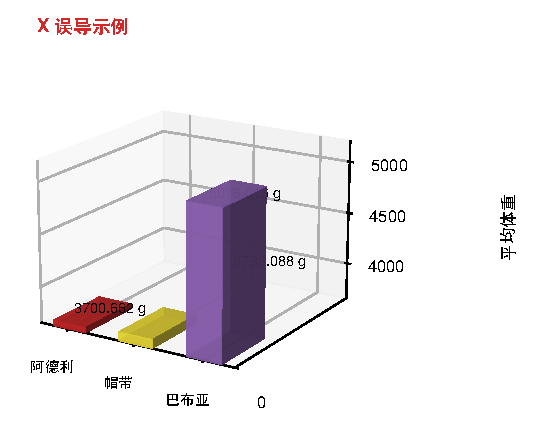
\includegraphics[width=0.49\linewidth]{figures/ch05/ch05-05-axis-bad-zh.pdf}\hfill
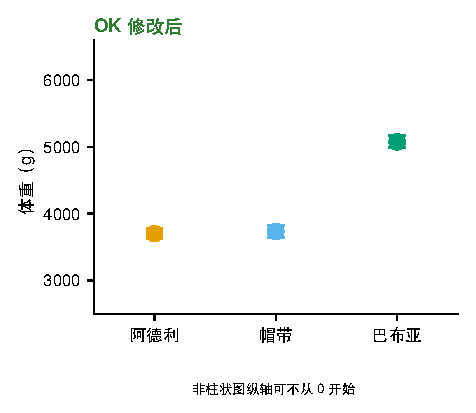
\includegraphics[width=0.49\linewidth]{figures/ch05/ch05-05-axis-good-zh.pdf}
\caption{同一组均值的误导画法与诚实画法（左为教学用错误示范）。左：3D 柱、纵轴从 $3650\ \text{g}$ 截断、彩虹配色、三位小数、缺少单位，使阿德利与帽带企鹅不足 1\% 的差异看起来像数倍差异。右：均值与 95\% 置信区间，纵轴有单位、刻度为整数。数据同图~\ref{fig:ch05-01}（$n = 342$）。}\label{fig:ch05-05}
\end{figure}

逐一剖析图~\ref{fig:ch05-05} 左图（\texttt{X 误导示例}）中的实际硬伤：
\begin{enumerate}
\item \textbf{截断柱状图纵轴夸大微小差异：}柱状图依赖**柱体距零基线的高度与面积**编码数值，纵轴必须从 $0$ 开始。左图将竖轴从 $3650\ \text{g}$ 截断起步：阿德利（$3700.7\ \text{g}$）与帽带（$3733.1\ \text{g}$）均值原本仅相差 $32.4\ \text{g}$（相对差异不足 $0.9\%$），减去 $3650\ \text{g}$ 基线后，红柱与黄柱的剩余高度变为 $50.7\ \text{g}$ 与 $83.1\ \text{g}$，视觉高度相差逾六成，而巴布亚（$5076.0\ \text{g}$）的紫柱更像高塔一样冲出视野。右图（\texttt{OK 修改后}）改用**均值点加 95\% 置信区间（点图）**：因为点图靠点在坐标轴上的位置而非柱体面积编码数值，纵轴可以从合理区间（$2500\text{--}6600\ \text{g}$）起步（图底专门注明“非柱状图纵轴可不从 0 开始”），前两个物种均值几乎齐平、置信区间大幅重叠的事实一目了然。
\item \textbf{3D 立体柱造成透视畸变与标签碰撞：}左图使用三维立体柱（\texttt{bar3d}），倾斜的柱顶让读者根本无法判断该拿前棱还是后棱去对齐右侧刻度（$4000, 4500, 5000$）；同时画面右下角多出无意义的纵深轴刻度“\texttt{0}”，右侧竖轴标题“平均体重”被挤到画幅边缘裁切不全，而半空中的数值标签 \texttt{5076.016 g} 与 \texttt{3733.088 g} 直接撞在紫色立体柱上。二维分组数据绝不应使用 3D 柱。
\item \textbf{多余小数位制造伪精度，且漏写单位：}野外称重最小刻度为 $25\ \text{g}$ 或 $50\ \text{g}$，左图却在柱顶标出毫克级的三位小数（\texttt{3700.662 g} 等）且竖轴无单位；右图删去图内冗余数字标签，纵轴规范标注“体重（g）”并采用整千刻度。
\end{enumerate}

第四类错误是连续矩阵与场数据中的\textbf{彩虹色图（\texttt{jet}）}。图~\ref{fig:ch05-07} 将 Mauna Loa 观测站 1959—2025 年共 67 个完整年 $\times$ 12 个月的 $\text{CO}_2$ 月均值排成 $67 \times 12$ 矩阵（不插值、不平滑，范围 $312.42\text{--}432.34\ \text{ppm}$），对比了 \texttt{jet} 彩虹色图与感知均匀色图 \texttt{viridis}。

\begin{figure}[htbp]\centering
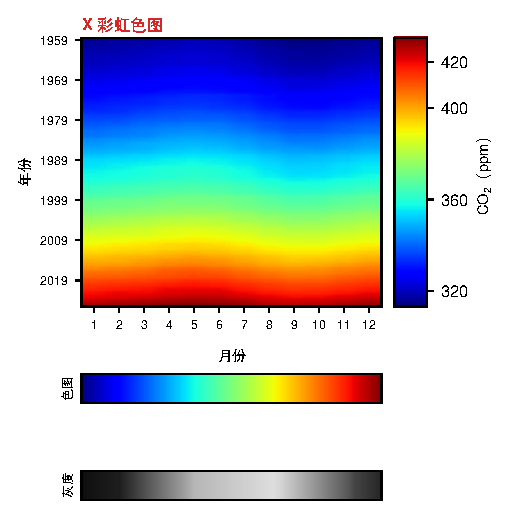
\includegraphics[width=0.49\linewidth]{figures/ch05/ch05-07-colormap-bad-zh.pdf}\hfill
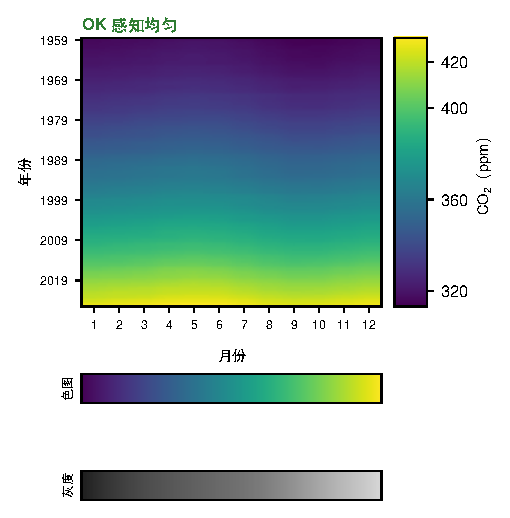
\includegraphics[width=0.49\linewidth]{figures/ch05/ch05-07-colormap-good-zh.pdf}
\caption{彩虹色图与感知均匀色图（左为教学用错误示范）。两张热图使用同一矩阵：Mauna Loa 1959—2025 年每月 $\text{CO}_2$ 均值。左 \texttt{jet} 色图在青、黄处出现数据中并不存在的“边界”，其灰度条亮度先升后降；右 \texttt{viridis} 的亮度单调上升，灰度打印后仍能读出高低顺序。}\label{fig:ch05-07}
\end{figure}

对比图~\ref{fig:ch05-07} 的左右两图及底部窄条可以看到：虽然 67 年来 $\text{CO}_2$ 浓度平稳上升，左图（\texttt{X 彩虹色图}）却在 1989 年前后的亮青色带和 2009 年前后的亮黄色带处造出两条刺眼的“假边界”；更严重的是，底部“灰度”转换条显示 \texttt{jet} 的感知亮度先升后降、两端（深蓝与深红）全暗，黑白打印后低值与高值混为一谈（Crameri 等，2020；Nuñez 等，2018）。右图（\texttt{OK 感知均匀}）改用 \texttt{viridis}（或针对重度色觉缺陷优化的 \texttt{cividis}），其灰度条从左至右单调变亮，既无假边界，黑白打印下也能准确读出长期上升与每年 5 月偏亮、9—10 月偏暗的季节波动。

在 \sdtool{sci-vis} 中遇到上述问题时，可直接发送如下修改指令：

\begin{Prompt}
1. 改为平面二维均值点 + 95% 置信区间图（若用柱状图，纵轴必须从 0 开始）；
   严禁使用 3D 立体柱；去掉三位小数标签，纵轴标题写为“体重（g）”，使用整数刻度。
2. 热图色图请将 jet 改为感知均匀的 viridis（或 cividis），色标注明单位“CO2（ppm）”。
\end{Prompt}

\section{色觉与灰度检查}

在北欧血统男性中约 8\% 有某种红绿色觉异常（最常见为第二色盲或绿色弱），其他人群中也有相当比例的读者受此影响（Wong，2011），加上黑白打印阅读场景，分组图绝不能只靠红绿颜色区分。

回到图~\ref{fig:ch05-08} 的面板 B–F：\textbf{面板 B} 将三个物种全部画成同样大小的实心圆点，仅靠红、绿、蓝三色区分；经基于生理学的色觉缺陷模型（Machado 等，2009）做第二色盲（deuteranopia）模拟后（\textbf{面板 C}），红色的阿德利点云与绿色的帽带点云连同各自的回归线、图例圆点一起塌缩成了难以分辨的黄褐色。相反，\textbf{面板 D} 同时采取三项措施：(1) 换用 Okabe–Ito 色觉安全配色（橙 \texttt{\#E69F00}、天蓝 \texttt{\#56B4E9}、蓝绿 \texttt{\#009E73}）；(2) 引入\textbf{形状冗余编码}（阿德利圆点 \texttt{o}、帽带三角形 \texttt{\^{}}、巴布亚正方形 \texttt{s}）；(3) 在各点云旁\textbf{直接标注物种名称}（实际排版时还应在终尺寸下检查标签位置，如面板 D 左上角相关系数文字紧邻高处散点、“巴布亚”贴近点云上沿，必要时可微调留白以免压点）。凭借这三重设计，无论在第二色盲模拟（\textbf{面板 E}）还是 CIELAB 亮度灰度图（\textbf{面板 F}）下，三个物种的点云与拟合线依然一目了然。

日常作图时，可将导出的图片上传至 \scidraw{} 图片检查（\sdtool{figure-checker}），一键完成灰度转换与色觉模拟检查；但须记住该工具仅覆盖技术检查，不能替代作者对科学逻辑（如面板 A 的辛普森悖论）的审核。

\section{贯穿案例：用 SciDraw AI 完成一张企鹅体重图}

现在我们把全章原则串联起来，完成开篇林悦的任务：基于公开数据集 \path{penguins.csv}，在论文“研究对象”一节和组会幻灯片中展示三种 \emph{Pygoscelis} 企鹅（阿德利 \emph{P.\ adeliae}、帽带 \emph{P.\ antarcticus}、巴布亚 \emph{P.\ papua}）繁殖成体的体重分布，以及每个物种内部雌雄体重的差别。明确科学边界：\textbf{本图仅作描述性形态展示，不做任何推断统计检验，不画星号或 $p$ 值。}

\textbf{第一步：独立复算期望值（准备核验标尺）。}按表~\ref{tab:ch05-dict} 规则，剔除 \texttt{sex} 或 \texttt{body\_mass\_g} 为 \texttt{NA} 的 11 行后保留 \textbf{$n = 333$} 行。在把数据交给 AI 之前，先用简单脚本或电子表格算出 6 个交叉子组的统计量（表~\ref{tab:ch05-case-expect}，SD 采用样本标准差 $\text{ddof}=1$；仅按物种合并的汇总量见前文表~\ref{tab:ch05-err}）。对比两表可见，分开雌雄后，每个物种内雄性均值都比雌性重 $412\text{--}805\ \text{g}$，且各亚组内的 SD（$269.4\text{--}362.1\ \text{g}$）比合并性别时的 SD（$384.3\text{--}504.1\ \text{g}$）明显缩小——说明原先混合分布的很大一部分离散度正是性别二态性造成的。

\begin{table}[htbp]\centering\footnotesize
\setlength{\tabcolsep}{4pt}
\renewcommand{\arraystretch}{1.15}
\caption{企鹅体重按“物种 $\times$ 性别”分组的核验期望值表（剔除缺失 11 行后，$n = 333$）。}\label{tab:ch05-case-expect}
\begin{tabularx}{\linewidth}{@{}llccY@{}}
\toprule
\textbf{物种（中文 / 英文与学名）} & \textbf{性别} & \textbf{记录数 $n$} & \textbf{均值 (g)} & \textbf{样本标准差 SD (g)} \\
\midrule
阿德利（Adelie, \emph{P.\ adeliae}） & 雌（female） & 73 & 3368.8 & 269.4 \\
阿德利（Adelie, \emph{P.\ adeliae}） & 雄（male）   & 73 & 4043.5 & 346.8 \\
帽带（Chinstrap, \emph{P.\ antarcticus}） & 雌（female） & 34 & 3527.2 & 285.3 \\
帽带（Chinstrap, \emph{P.\ antarcticus}） & 雄（male）   & 34 & 3939.0 & 362.1 \\
巴布亚（Gentoo, \emph{P.\ papua}） & 雌（female） & 58 & 4679.7 & 281.6 \\
巴布亚（Gentoo, \emph{P.\ papua}） & 雄（male）   & 61 & 5484.8 & 313.2 \\
\bottomrule
\end{tabularx}
\end{table}

\textbf{第二步：编写任务书并按向导进入绘图。}先把下面的任务书保存在自己的文档里；再打开 \scidraw{} 科研绘图向导（\sdtool{figure-workflow}），选“数据图”，从第 1 步“上传数据并绘图”进入科学可视化（\sdtool{sci-vis}）：

\begin{Prompt}
【研究问题】三种 Pygoscelis 企鹅的体重分布有何不同？每个物种内，雌雄体重相差多少？
【用途与读者】论文“研究对象”一节的描述性图 + 组会幻灯片；读者为生态学同行。
             单栏宽约 85 mm；同一张图另存一版供幻灯片使用。
【数据来源】真实公开数据：palmerpenguins v0.1.0 的 penguins.csv（CC0），
             Palmer Station LTER，2007–2009。
【字段与单位】species（分组）、sex（分组）、body_mass_g（体重，g）。其余列本图不用。
【观测单位与样本量】每行是一条测量记录。剔除 sex 或 body_mass_g 为 NA 的行（共 11 行），
             保留 333 行。每组 n 必须在图上可见。
【配对关系】无。不同记录之间不配对，不要连线。
【希望表达】分布与比较：每个物种内雌雄并排；物种按 Adelie、Chinstrap、Gentoo 排列。
【汇总与误差条】显示全部原始点（只在横向抖动，纵向值不变）；每组叠加均值 ± 1 SD。
             不做显著性检验，不画星号或 p 值。
【不允许的处理】不编造、删除或静默修改任何数值；不剔除“离群值”；不插补缺失值。
【标签与输出】纵轴“体重（g）”，整数刻度；横轴为物种；性别用空心/实心标记区分，
             颜色区分物种并对色觉异常友好；图例写明“均值 ± SD”。输出 PNG 和 PDF。
【验收】六组 n 依次为 73、73、34、34、58、61；六个均值与我核对的数值表一致（见数据字典附表）。
\end{Prompt}

\textbf{第三步：上传数据与排查初稿问题。}在科学可视化（\sdtool{sci-vis}）上传 \path{penguins.csv}（支持 CSV、TSV、TXT、XLSX、XLS 与粘贴表格；Excel 只读首个工作表），首先核对界面显示的行列信息是否为 344 行 $\times$ 8 列。平台对上传数据做哈希、字节数与行数校验，并提供“下载原始数据”供取回比对，保证画的是你上传的那份数据；但这不证明统计选择正确。在“绘图要求”输入框粘贴任务书要求后生成初稿，对照表~\ref{tab:ch05-case-expect} 逐项排查五类常见初稿问题：(1) 画成均值柱 + 不明误差线（常为 SEM）；(2) 性别被合并，或 \texttt{sex} 为 \texttt{NA} 的记录被当作第三个性别组“\texttt{NA}”；(3) 柱状图纵轴从非零值截断；(4) 均值标签带 1–3 位小数；(5) 颜色为红/绿或默认彩色，未配空心/实心标记。

\textbf{第四步：分步下达修改指令与历史版本恢复。}在会话底部继续输入修改指令，一次只改一类问题。第一轮修改指令 M1（图型与数据清理）：

\begin{Prompt}
请改为散点图：每个点是一条测量记录，横轴为物种（Adelie、Chinstrap、Gentoo 依次排列），
每个物种内雌性在左、雄性在右。点只在横向轻微抖动（宽度不超过组间距的 15%），纵向数值不变。
剔除 sex 或 body_mass_g 为 NA 的行，不要出现“NA”组。不要画柱子。其余设置保持不变。
\end{Prompt}

第二轮修改指令 M2（汇总量与样本量标注）：

\begin{Prompt}
在每组点的右侧叠加均值（短横线）和均值 ± 1 个标准差（SD，样本标准差）的竖线。
在每组下方标注样本量，例如“n = 73”。图例中写明“横线：均值；竖线：± 1 SD”。
不要添加显著性星号、p 值或检验结果。只改这两项，其余保持不变。
\end{Prompt}

第三轮修改指令 M3（坐标轴、整数刻度与色觉友好配色）：

\begin{Prompt}
纵轴标题为“体重（g）”，范围 2500–6500，刻度间隔 500，刻度为整数，不显示小数。
物种颜色使用对色觉异常友好的配色：Adelie 橙 #E69F00，Chinstrap 天蓝 #56B4E9，
Gentoo 蓝绿 #009E73；雌性空心圆，雄性实心圆。不要改变物种顺序和任何数值。
\end{Prompt}

注意：对话式修改不能保证“锁定”未提及的元素。若执行 M3 后发现意外改变了物种排列顺序或点的位置，不要在错图上继续叠加修补，而应立即点击“恢复上一版”（界面提示“已恢复上一版。”，也可从侧栏“历史记录”选回上一版），再把 M3 拆成两条更窄的指令（先改坐标轴，确认无误后再改配色与标记）。每次修改后都必须重新检查原本没要求改的部分。

\textbf{第五步：终稿核验、图注与交付文件夹。}平台后台用声明式图表或 Python 两条路径绘图，当前界面不提供完整代码下载，且声明式路径下导出的 PDF/EPS 可能是栅格包装（不要直接称为可编辑矢量；部分常见图型可导出原生 Excel 图表）。因此，我们用独立脚本复算并绘制标准对照终稿（图~\ref{fig:ch05-02}），对照表~\ref{tab:ch05-case-expect} 逐项核验：横轴依次为阿德利、帽带、巴布亚，每物种内左雌（空心圆）右雄（实心圆），点仅横向抖动；每组点右侧黑色短横线与竖线准确对应均值 $\pm 1\ \text{SD}$；横轴物种名下方分两行标出样本量（上行对应左侧雌性组：$n = 73, 34, 58$；下行对应右侧雄性组：$n = 73, 34, 61$，合计 333，无 \texttt{NA} 组）。

\begin{figure}[htbp]\centering
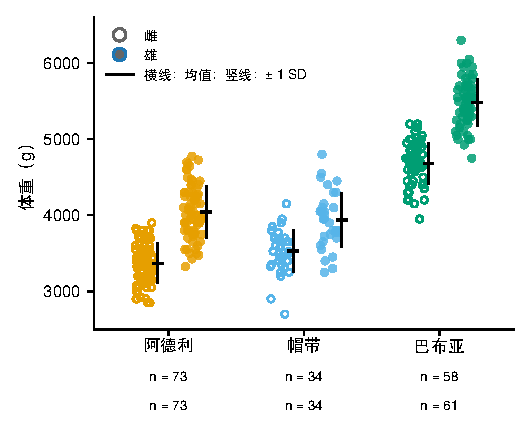
\includegraphics[width=0.68\linewidth]{figures/ch05/ch05-02-case-final-zh.pdf}
\caption{三种企鹅繁殖成体的体重（按物种与性别）。每个点为一条测量记录（Palmer Station LTER，2007—2009；palmerpenguins v0.1.0，CC0）。剔除性别或体重缺失的 11 条记录后 $n = 333$，各组 $n$ 标于横轴下方。横线为均值，竖线为均值 $\pm 1\ \text{SD}$（样本标准差）。点在横向随机抖动以减少重叠，纵向数值未改变。本图为描述性展示，未进行统计检验。}\label{fig:ch05-02}
\end{figure}

若把终稿交给 \sdtool{figure-legend} 起草图注，作者必须亲手补齐数据来源与许可、剔除 11 条缺失记录后的 $n = 333$、均值 $\pm 1\ \text{SD}$ 含义、“仅横向抖动”及“未进行统计检验”说明。最后将全套产物按如下结构归档交付（本章示例图由确定性脚本生成，提示词与核验记录见本书仓库）：

\begin{Prompt}
penguin-mass-figure/
  source/   penguins.csv、penguins-README.md、SHA-256.txt
  brief/    任务书.txt、数据字典.md、期望值表.csv
  drafts/   scivis-v1.png … scivis-v4.png、修改指令.md（每轮输入原文 + 发现的问题）
  check/    独立脚本复算输出 check.json、figure-checker 报告
  final/    figure-5-2.png、figure-5-2.pdf、图注-中.txt、caption-en.txt、AI 使用说明.txt
\end{Prompt}

\section{AI 在这一步能做什么与不能做什么}

表~\ref{tab:ch05-02} 汇总了数据可视化各环节中 AI 工具的能力边界与作者必须核对的事项。

\begin{table}[htbp]\centering\footnotesize
\setlength{\tabcolsep}{3pt}
\renewcommand{\arraystretch}{1.15}
\caption{数据可视化各环节中 AI 能做什么、不能做什么与作者要核对的内容。}\label{tab:ch05-02}
\begin{tabularx}{\linewidth}{@{}>{\raggedright\arraybackslash}p{18mm}YYY@{}}
\toprule
\textbf{环节} & \textbf{AI（\scidraw{} 科学可视化）能做} & \textbf{不能做 / 不应交给它} & \textbf{作者要核对} \\
\midrule
读取数据 & 解析 CSV、TSV、TXT、XLSX、XLS 与粘贴表格；校验上传数据的哈希、字节数与行数 & 知道哪一行属于同一个体、哪一列是配对键；判断缺失值的原因；Excel 只读首个工作表 & 行数、列名、NA 数与原始文件一致；观测单位写进任务书 \\
选择图型 & 按指令画散点、箱线、点线、折线、热图等；根据描述提出候选 & 理解研究设计（独立/配对/重复测量）除非你写明；当前界面不展示图型推荐理由 & 图型与研究设计匹配；全部原始点是否需要显示 \\
汇总与误差线 & 计算均值、SD、SEM、CI 并画出 & 替你决定该用哪种误差线；保证统计检验适用 & 误差线类型写在图例和图注；$n$ 与图上一致；无未要求的星号/$p$ 值 \\
多轮修改 & 在会话中按指令改图型、标签、颜色、轴；从历史图继续；恢复上一版 & 保证只改你要求的部分；“锁定”某个元素 & 每轮修改后重新检查没要求改的部分（顺序、数值、范围） \\
颜色与可读性 & 应用指定调色板与期刊栏宽样式；图片检查中做灰度与色觉模拟 & 判断颜色是否承载了科学含义；技术检查不代表科学审核 & 色觉模拟/灰度下分组仍可区分；色图与数据类型（顺序/发散/分类）匹配 \\
导出 & 下载 PNG、TIFF、PDF、EPS；下载原始数据；部分图型导出原生 Excel 图表 & 当前界面不提供完整绘图代码下载；PDF/EPS 不一定是可编辑矢量 & 打开导出文件确认尺寸、字体和是否栅格；源数据哈希与本地一致 \\
图注 & \sdtool{figure-legend} 根据图片起草描述 & 知道 $n$、剔除规则、误差线含义、数据来源（它只读图片） & 补齐数据来源、$n$、缺失值处理、误差线类型、是否检验 \\
\bottomrule
\end{tabularx}
\end{table}

\section{本章检查清单}

\begin{itemize}
\item 每一行代表什么已写在任务书里；“记录数”和“个体数”没有混用。
\item 缺失值怎么处理写明了；图上没有“NA”组；剔除的行数写进图注。
\item 图型与研究设计匹配：配对数据保留配对，时间轴是连续数值，分组变量在图上可见。
\item $n \le$ 几十时显示全部原始点；抖动只在横向。
\item 误差线类型（SD / SEM / 95\% CI）写在图例或图注里，$n$ 与图一致。
\item 柱状图纵轴从 0 开始；非柱状图的纵轴范围有理由，且不夸大差异。
\item 没有双纵轴、3D 柱、伪精度的小数。
\item 连续数据用感知均匀色图；分组颜色经过色觉模拟和灰度检查，并有形状或标注冗余。
\item 图上所有数字已与独立复算（脚本或表格软件）对照。
\item 保存了：原始数据及其哈希、任务书、每轮指令与截图、终稿、图注、核对记录。
\item 模拟数据在图或图注中标为“模拟教学数据”。
\end{itemize}

\section{练习}

\begin{enumerate}
\item \textbf{读表与选图（纸笔）：}给出 Palmer Penguins 的 \texttt{flipper\_length\_mm} 与 \texttt{island}。写一份数据字典（含 NA 数），统计各岛的物种构成（Torgersen 52 条阿德利；Biscoe 44 条阿德利 + 124 条巴布亚；Dream 56 条阿德利 + 68 条帽带），判断“比较三个岛上的鳍肢长度”为什么会与物种混杂（巴布亚只在 Biscoe、帽带只在 Dream），并提出一个不误导的图（例如按岛分面、按物种着色）。
\item \textbf{\scidraw{} 实操：}在 \sdtool{sci-vis} 上传 \texttt{paired-example.csv}，先只输入“画一张前后比较图”，记录初稿；再用本章图~\ref{fig:ch05-03} 的思路，通过对话分别得到配对点线图与差值图（纵轴含 0），至少使用一次“恢复上一版”。提交：每轮输入原文、截图，以及一张核对表（8 个差值逐一核对，\texttt{SIM04} $= -1$）。
\item \textbf{改错：}用本章 $\text{CO}_2$ 快照，自己制作一张“彩虹色 + 双纵轴”的错误图，再写出三条可以直接发给 AI 的修改指令把它改正；说明你如何确认修改后数值没有变（例如对比年均值表）。
\end{enumerate}

\section*{参考文献}

\begin{itemize}
\item Allen M, Poggiali D, Whitaker K, Marshall TR, Kievit RA. Raincloud plots: a multi-platform tool for robust data visualization. \emph{Wellcome Open Research}. 2019;4:63. \url{https://doi.org/10.12688/wellcomeopenres.15191.1}
\item ColorBrewer 2.0: color advice for cartography and scientific visualization. \url{https://colorbrewer2.org/}
\item Crameri F, Shephard GE, Heron PJ. The misuse of colour in science communication. \emph{Nature Communications}. 2020;11:5444. \url{https://doi.org/10.1038/s41467-020-19160-7}
\item Cumming G, Fidler F, Vaux DL. Error bars in experimental biology. \emph{Journal of Cell Biology}. 2007;177(1):7--11. \url{https://doi.org/10.1083/jcb.200611141}
\item Gorman KB, Williams TD, Fraser WR. Ecological sexual dimorphism and environmental variability within a community of Antarctic penguins (genus \emph{Pygoscelis}). \emph{PLoS ONE}. 2014;9(3):e90081. \url{https://doi.org/10.1371/journal.pone.0090081}
\item Horst AM, Hill AP, Gorman KB. palmerpenguins: Palmer Archipelago (Antarctica) penguin data (v0.1.0) [R package]. Zenodo; 2020. \url{https://doi.org/10.5281/zenodo.3960218}
\item Keeling CD. The concentration and isotopic abundances of carbon dioxide in the atmosphere. \emph{Tellus}. 1960;12(2):200--203. \url{https://doi.org/10.3402/tellusa.v12i2.9366}
\item Krzywinski M, Altman N. Points of significance: error bars. \emph{Nature Methods}. 2013;10(10):921--922. \url{https://doi.org/10.1038/nmeth.2659}
\item Lan X, Keeling R. Trends in atmospheric carbon dioxide: Mauna Loa monthly mean data. NOAA Global Monitoring Laboratory and Scripps Institution of Oceanography. \url{https://gml.noaa.gov/ccgg/trends/data.html}
\item Machado GM, Oliveira MM, Fernandes LAF. A physiologically-based model for simulation of color vision deficiency. \emph{IEEE Transactions on Visualization and Computer Graphics}. 2009;15(6):1291--1298. \url{https://doi.org/10.1109/TVCG.2009.113}
\item Nu\~nez JR, Anderton CR, Renslow RS. Optimizing colormaps with consideration for color vision deficiency to enable accurate interpretation of scientific data. \emph{PLoS ONE}. 2018;13(7):e0199239. \url{https://doi.org/10.1371/journal.pone.0199239}
\item Okabe M, Ito K. Color Universal Design (CUD): how to make figures and presentations that are friendly to colorblind people. \url{https://jfly.uni-koeln.de/color/}
\item Rougier NP, Droettboom M, Bourne PE. Ten simple rules for better figures. \emph{PLoS Computational Biology}. 2014;10(9):e1003833. \url{https://doi.org/10.1371/journal.pcbi.1003833}
\item Weissgerber TL, Milic NM, Winham SJ, Garovic VD. Beyond bar and line graphs: time for a new data presentation paradigm. \emph{PLOS Biology}. 2015;13(4):e1002128. \url{https://doi.org/10.1371/journal.pbio.1002128}
\item Wong B. Points of view: color blindness. \emph{Nature Methods}. 2011;8(6):441. \url{https://doi.org/10.1038/nmeth.1618}
\end{itemize}

% TODO: 待补充 SciDraw AI 科学可视化（/sci-vis）实测界面与迭代截图（磁盘上暂未生成，故正文未插）：
% - figures/ch05/ch05-scivis-v1.png（/sci-vis 初稿截图）
% - figures/ch05/ch05-scivis-v2.png … ch05-scivis-v4.png（多轮对话修改与恢复上一版截图）
